\documentclass[crop,tikz]{standalone}
\usetikzlibrary{backgrounds}
\colorlet{blue}{cyan}
\tikzset{
  inverted/.style = {
    color=white,
    background rectangle/.style={fill},
    show background rectangle
  }
}

\usepackage{amsmath,marvosym}
\tikzset{>=latex}
\usetikzlibrary{decorations.markings,positioning,arrows}

\begin{document}
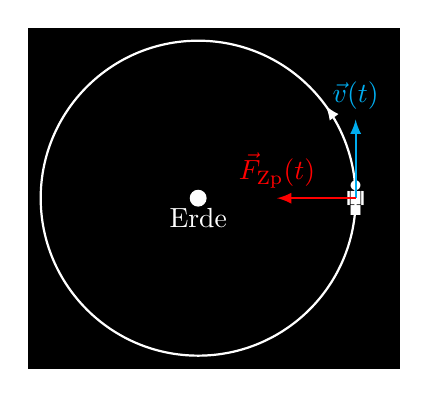
\begin{tikzpicture}[inverted,scale=2]
  \draw[fill] (0,0) circle (0.05) node[below] {Erde};
  \draw[thick,
        decoration={markings, mark=at position 0.1 with {\arrow{>}}},
        postaction={decorate}
        ] (0,0) circle (1);
  \coordinate (P) at (1,0);
  \node at (P) {\LARGE\Gentsroom};
  \draw[->,blue,thick] (P) -- ++(0,0.5) node[above] {$\vec{v}(t)$};
  \draw[->,red,thick] (P) -- ++(-0.5,0) node[above] {$\vec{F}_\text{Zp}(t)$};
\end{tikzpicture}
\end{document}
